\documentclass[../sections/subsections/modelos_continuos.tex]{subfiles}

\newcounter{mycounter}

    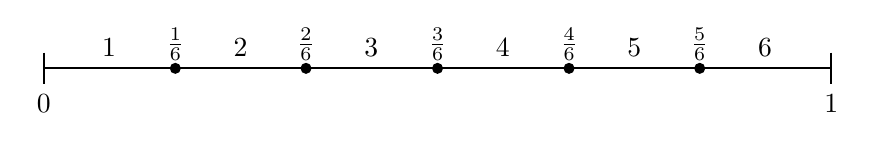
\begin{tikzpicture}[
dot/.style = {circle, fill=black,inner sep=0pt, minimum size=4pt},
every label/.append style = {inner sep=0pt},
    thick      
                        ]
\draw ( 0,0.2) -- + (0,-0.4) node[below] {0};
\draw (10,0.2) -- + (0,-0.4) node[below] {1};
%
\draw[thick] (0,0) -- node[below=2mm] {} + (10,0);
%
\setcounter{mycounter}{1}
%
\foreach \p in {0.167, 0.333, 0.5, 0.667, 0.833}
{
    \node[dot,label={$\frac{\themycounter{}}{6}$}] at (10*\p,0) {};
    \stepcounter{mycounter}
}

\setcounter{mycounter}{1}
\foreach \p in {0.083, 0.25, 0.416, 0.583, 0.75, 0.916}
{
    \node[label={$\themycounter{}$}] at (10*\p,0) {};
    \stepcounter{mycounter}
}

\end{tikzpicture}